\label{fs-drifting}

An important special case of grouping with $Window Size = 2$  provides for realization of stateful calculations with drifting state technique manifested in section~\ref{motivation-section}. Indeed, consider a map operation that follows the grouping and sends its output to the grouping input. This map operation receives a pair of its previous output considered as the state object, and new incoming item from the source stream. The map operation calculates new state object and sends it back as the grouping input. 

As an example, let us demonstrate a generic MapReduce transformation. The map stage of MapReduce can be expressed in terms of our map operation. The generic reduce stage can be presented as

\begin {tabbing}
1234\=1234\= \kill
{\bf for} $mapped \in values$ {\bf do}   \\
\>$accumulator$ := combine ($mapped$, $accumulator$); \\
{\bf end for} \\
{\bf return } $accumulator$;
\end {tabbing}

The {\it accumulator} is an explicit state that should be kept between subsequent iterations. To implement reduce stage we apply the drifting state technique and make the accumulator value a part of the stream. Figure~\ref{mapreduce-graph-figure} shows a generic graph for the MapReduce transformation. Map and reduce stages are highlighted with a dashed line. 

\begin{figure}[ht]
  \centering
  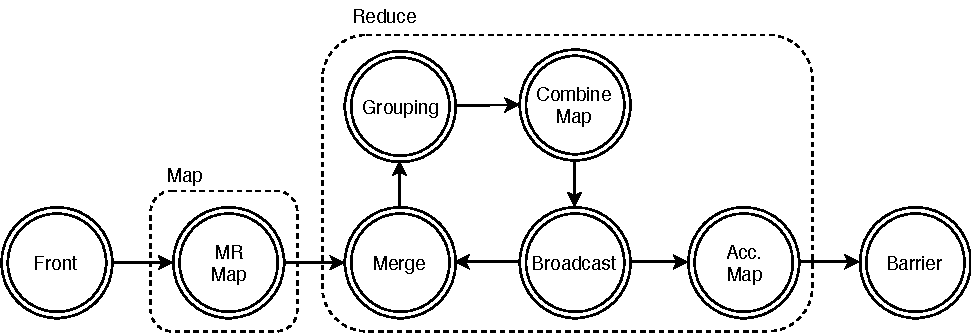
\includegraphics[width=0.6\textwidth]{pics/mapreduce}
  \caption{Logical graph for MapReduce transformations}
  \label {mapreduce-graph-figure}
\end{figure}

There are four types of data items in this stream: {\em input}, {\em mapped}, {\em accumulator}, and {\em reduced}. The operations of the stream have the following purposes:

\begin{itemize}
  \item The first map operation outputs mapped items according to map stage of MapReduce model.
  
  \item The grouping with $WindowSize=2$ groups the $accumulator$ with next $mapped$ item. 
  
  \item The combine map produces new state of $accumulator$ to be sent to grouping.
  
  \item The final map converts $accumulator$ into final reduce output.
\end{itemize}

Ordering rules  guarantee that each $accumulator$  item always arrives at the grouping right before next not yet combined mapped item. The cycle gives the ability for new accumulator items to get back in the grouping operation. Thereby, the stream reacts to each input item by generating new reduced item, which contains the actual value of the reduce stage.
